\renewcommand\thesection{\Alph{section}}
\renewcommand\thesubsection{\thesection.\arabic{subsection}}
\setcounter{section}{0}
\section{Entrega acumulada A}

\setcounter{subsection}{1}
\subsection{Menú con funcionalidades de edición y eliminación de elementos}

A través del menú en la interfaz de consola de comandos (CLI), también nos permite editar y eliminar datos relacionados a los Cursos y los Alumnos. Específicamente, se puede:

\begin{itemize}
    \item Editar o eliminar alumnos: Se pueden modificar los datos del alumno (exceptuando el RUT). No así los datos del apoderado, ya que es una funcionalidad que estará disponible en las entregas siguientes. También se pueden eliminar los alumnos, lo que provoca a su vez que se elimine del sistema al apoderado que tenga asociado.
    \Shell{Menú alumnos}{contents/code/salida8.txt}

    \item Asignar nuevo profesor jefe a curso: Se puede modificar un curso, asignándole un nuevo profesor jefe y eliminando al anterior.
    \item Eliminar curso: El programa permite la eliminación completa de un curso, la que provocará también la eliminación de los datos del profesor, alumnos, y por consiguiente, de los apoderados.
    \Shell{Menú cursos}{contents/code/salida9.txt}
\end{itemize}

\subsection{Se debe generar un reporte en archivo txt que considere mostrar datos de las 2 colecciones anidadas (ej: csv)}

El programa permite la generación de reportes en formato CSV (separados por comas), tanto en la interfaz de linea de comandos, como en la interfaz gráfica. Los reportes que se pueden generar son los siguientes:

\begin{itemize}
    \item Lista del curso: Este archivo CSV contendrá los datos de los alumnos de un curso en específico, entregado por el usuario.
    \item Tabla de cursos: Este archivo CSV contendrá los datos generales de todos los cursos a los que el programa tiene acceso. Esta tabla, además de mostrar los datos del curso mismo, muestra datos generales del profesor jefe a cargo del mismo.
\end{itemize}

\Shell{Menú reportes}{contents/code/salida10.txt}

\begin{figure}[h]
    \centering
    \frame{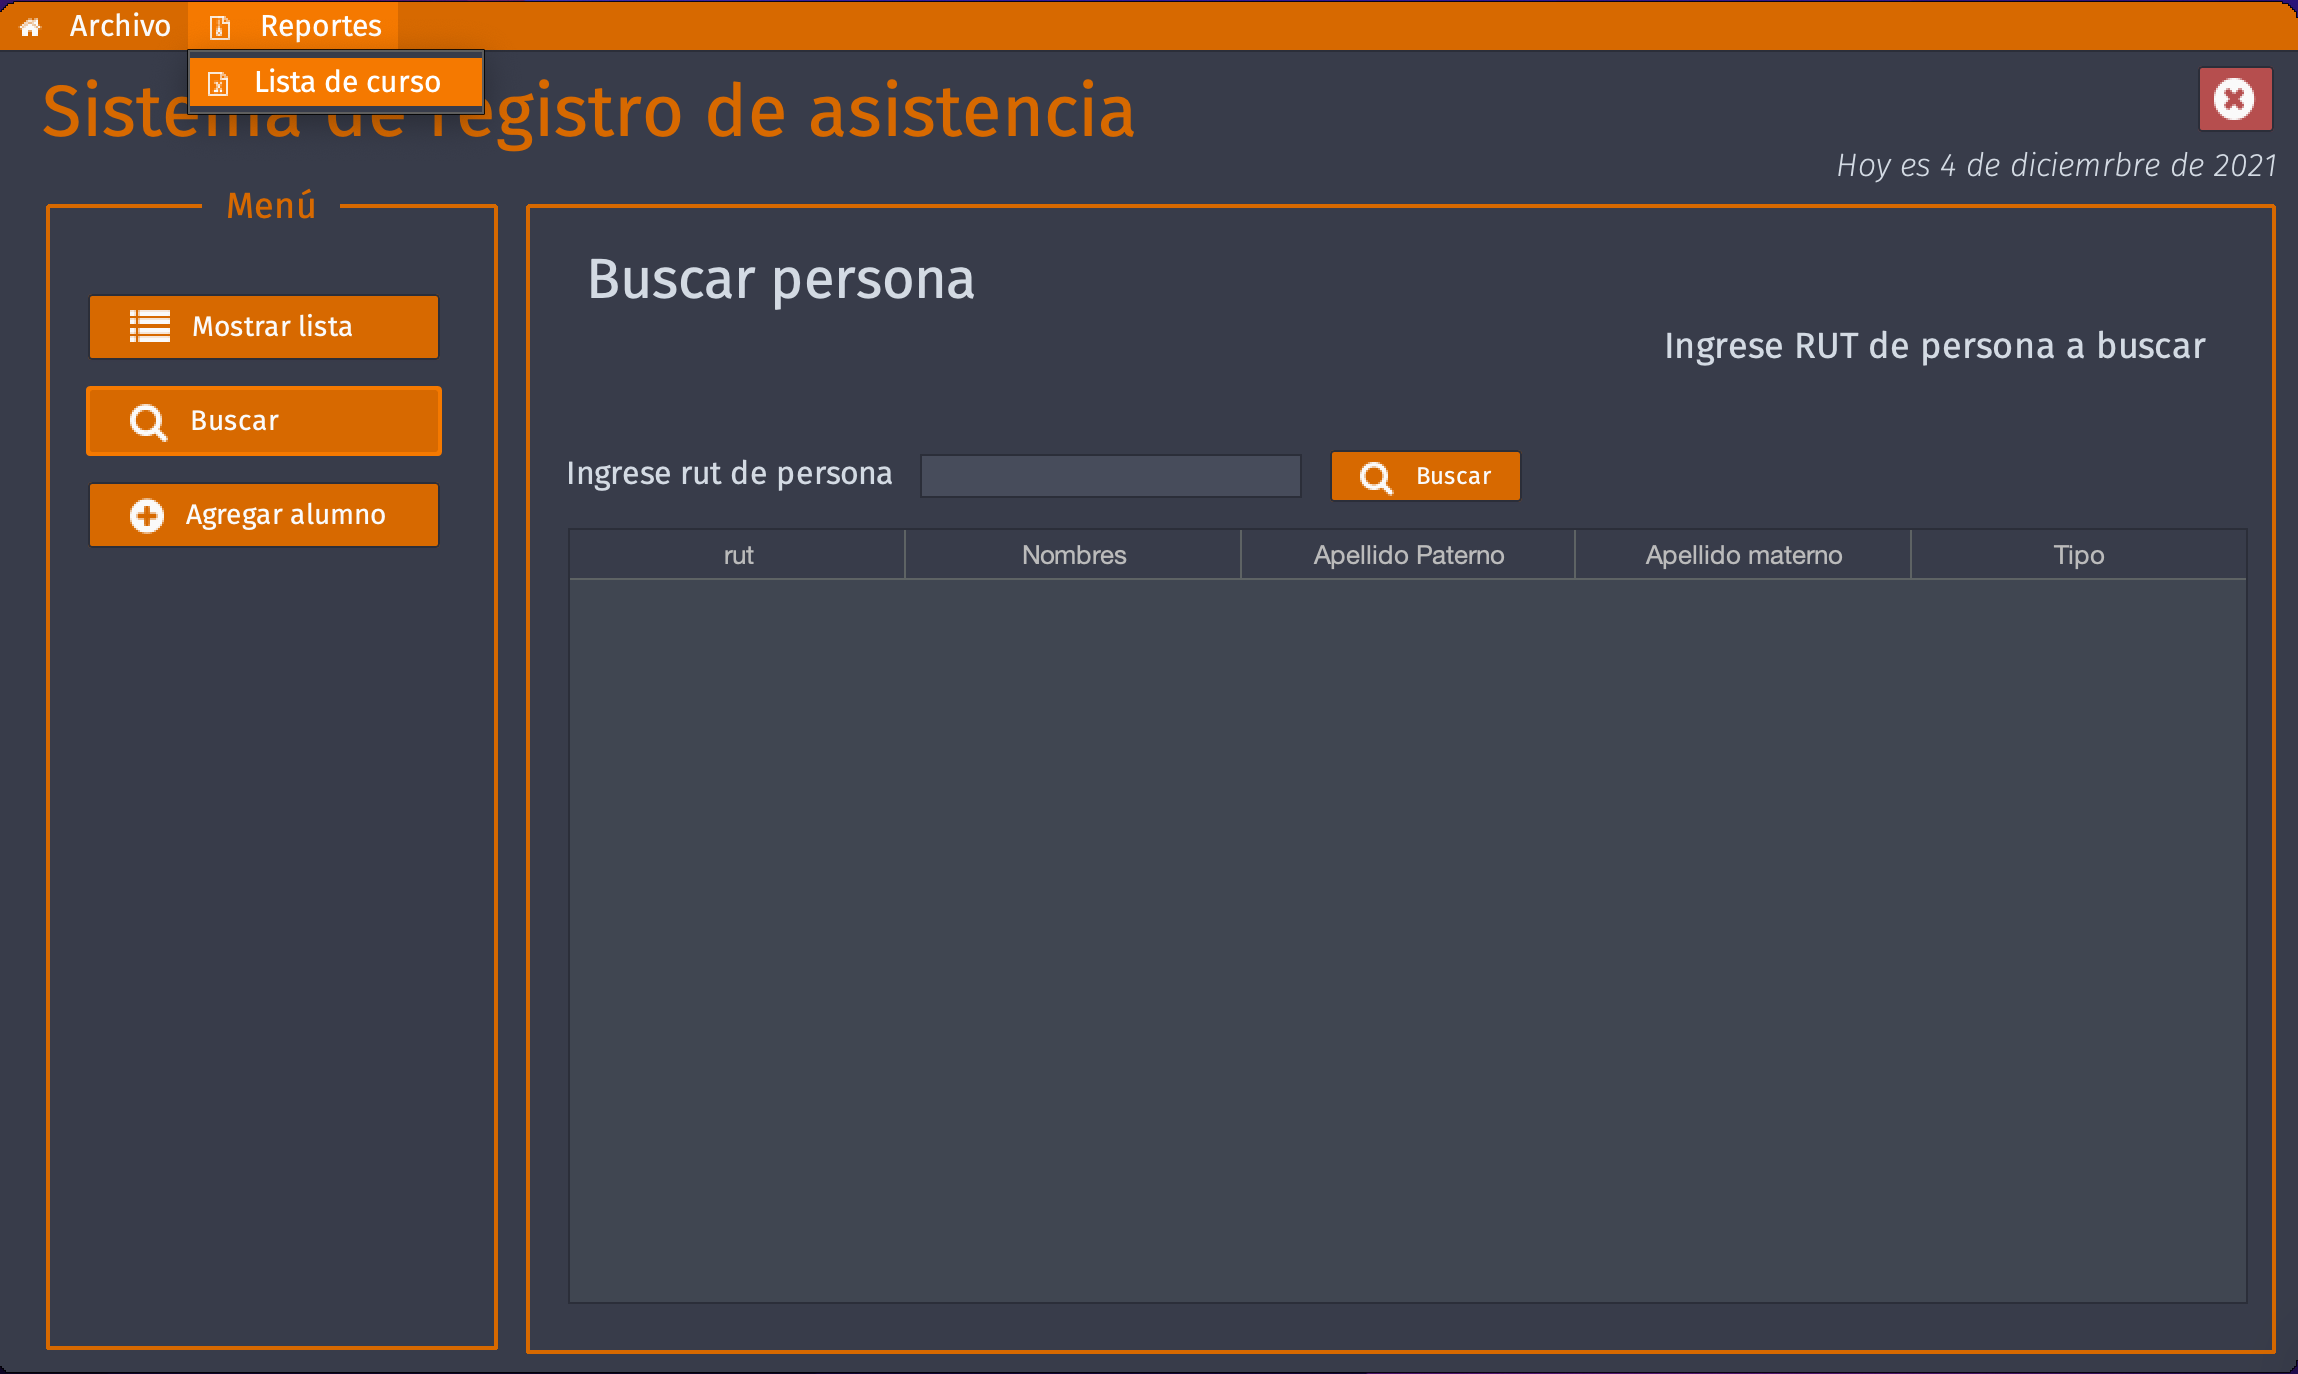
\includegraphics[width=0.95\textwidth]{contents/img/gui/img14}}
\end{figure}

\begin{figure}
    \centering
    \begin{subfigure}{0.5\textwidth}
        \centering
        \frame{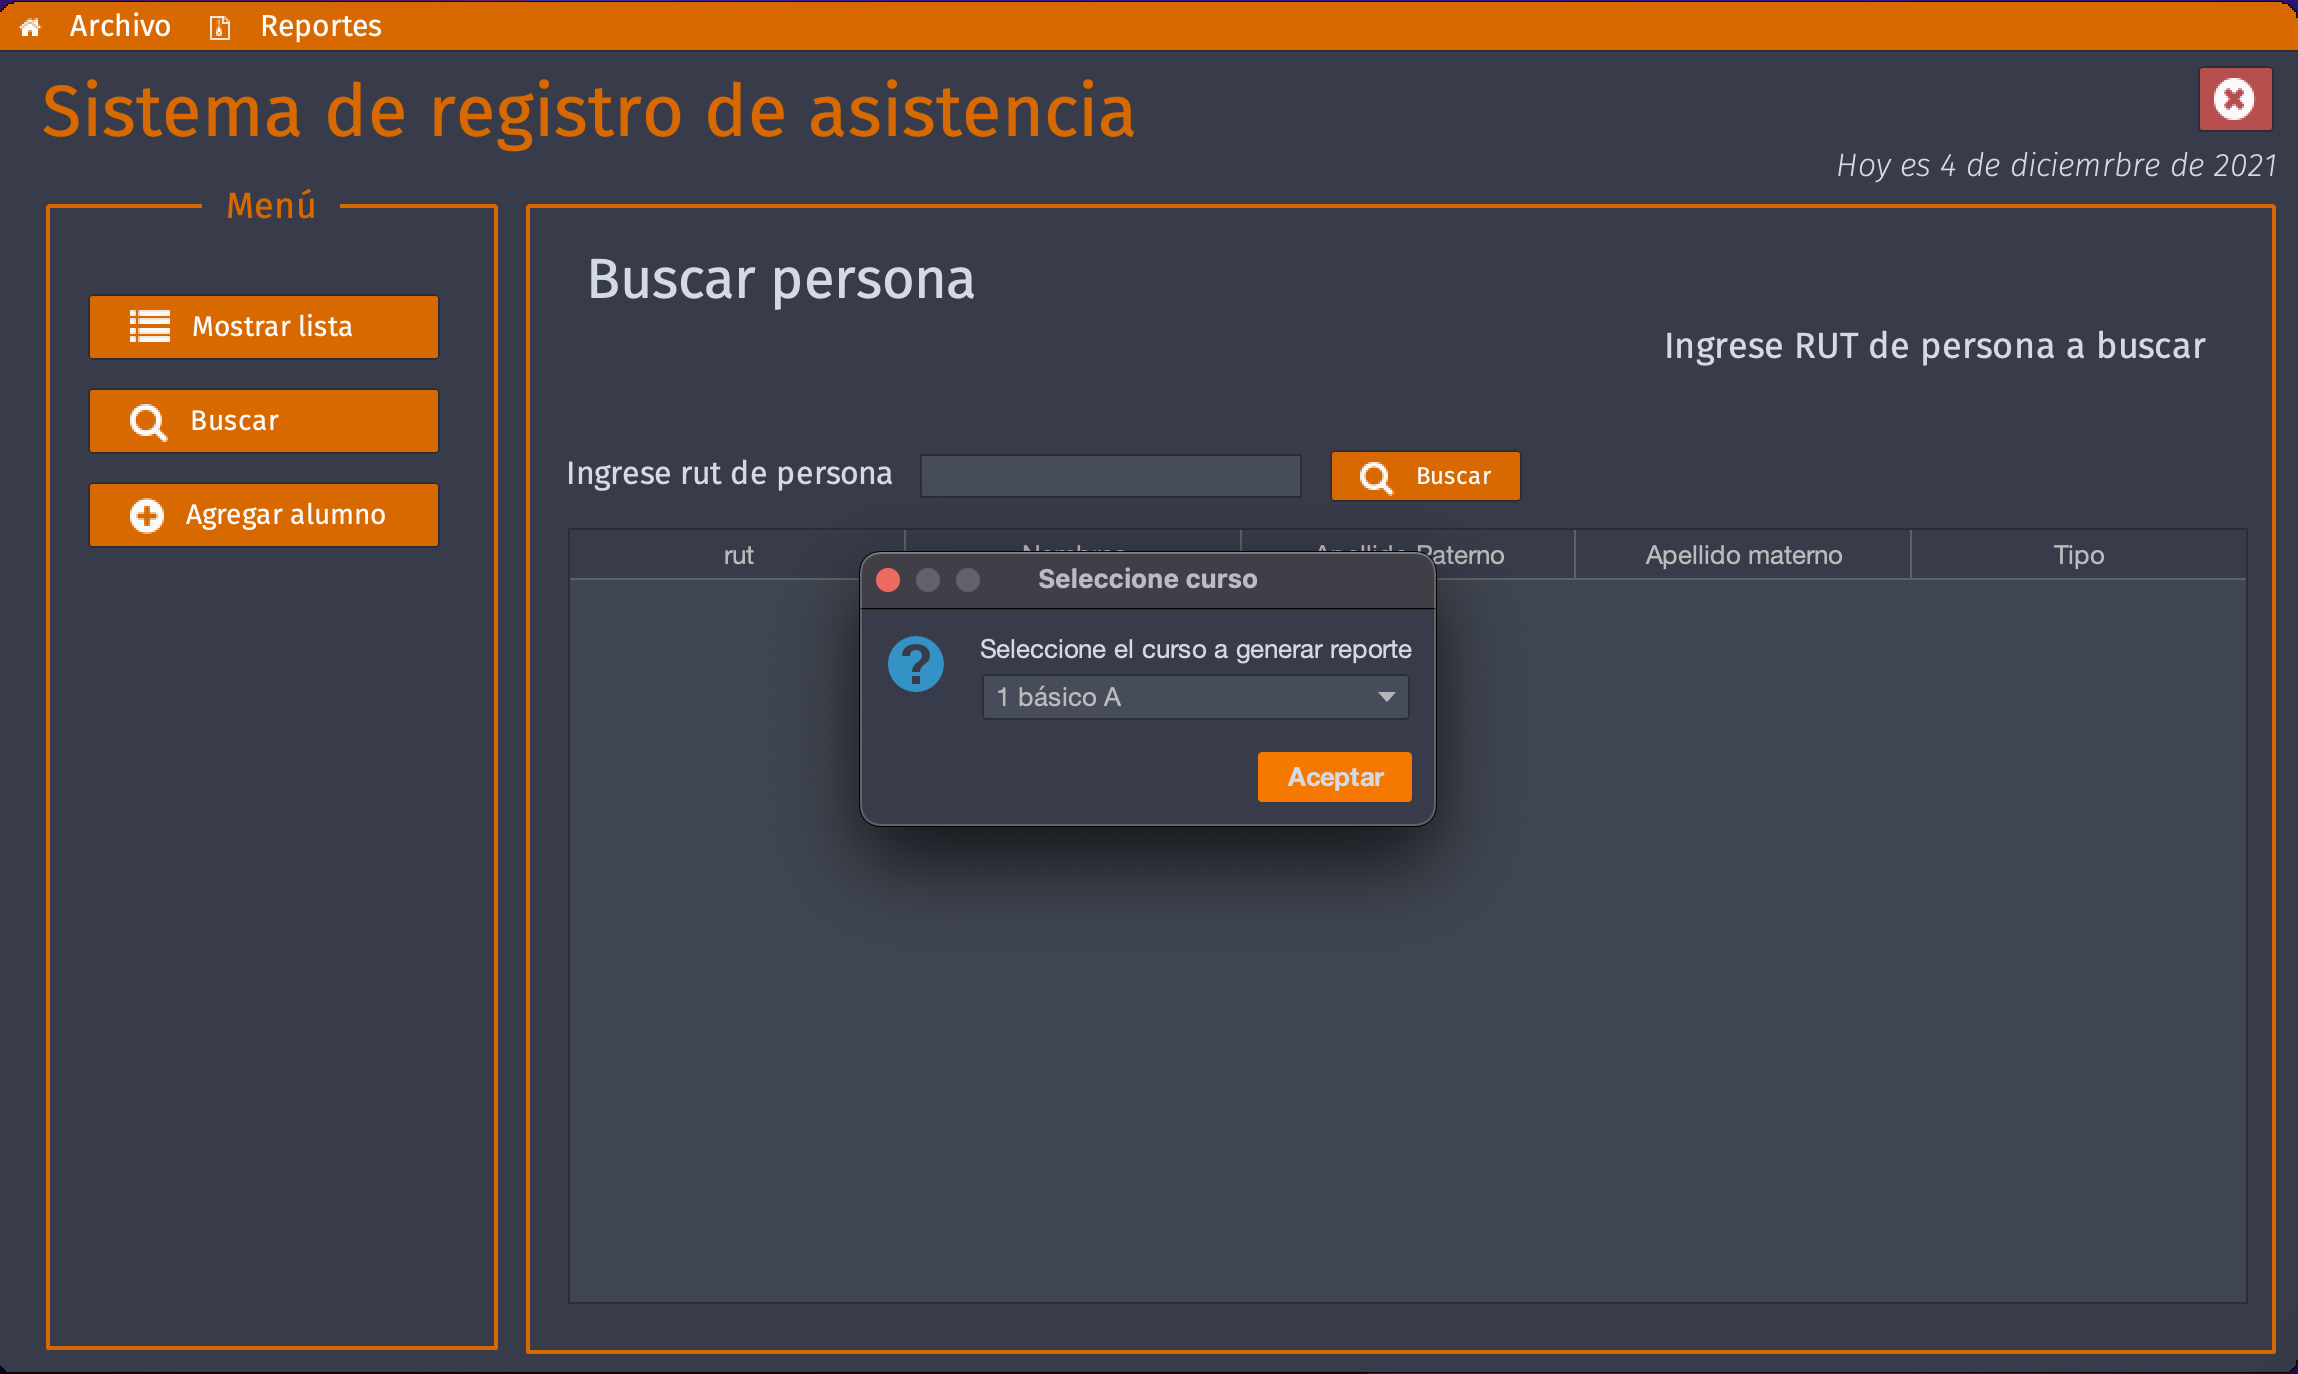
\includegraphics[width=0.95\linewidth]{contents/img/gui/img15}}
    \end{subfigure}%
    \begin{subfigure}{0.5\textwidth}
        \centering
        \frame{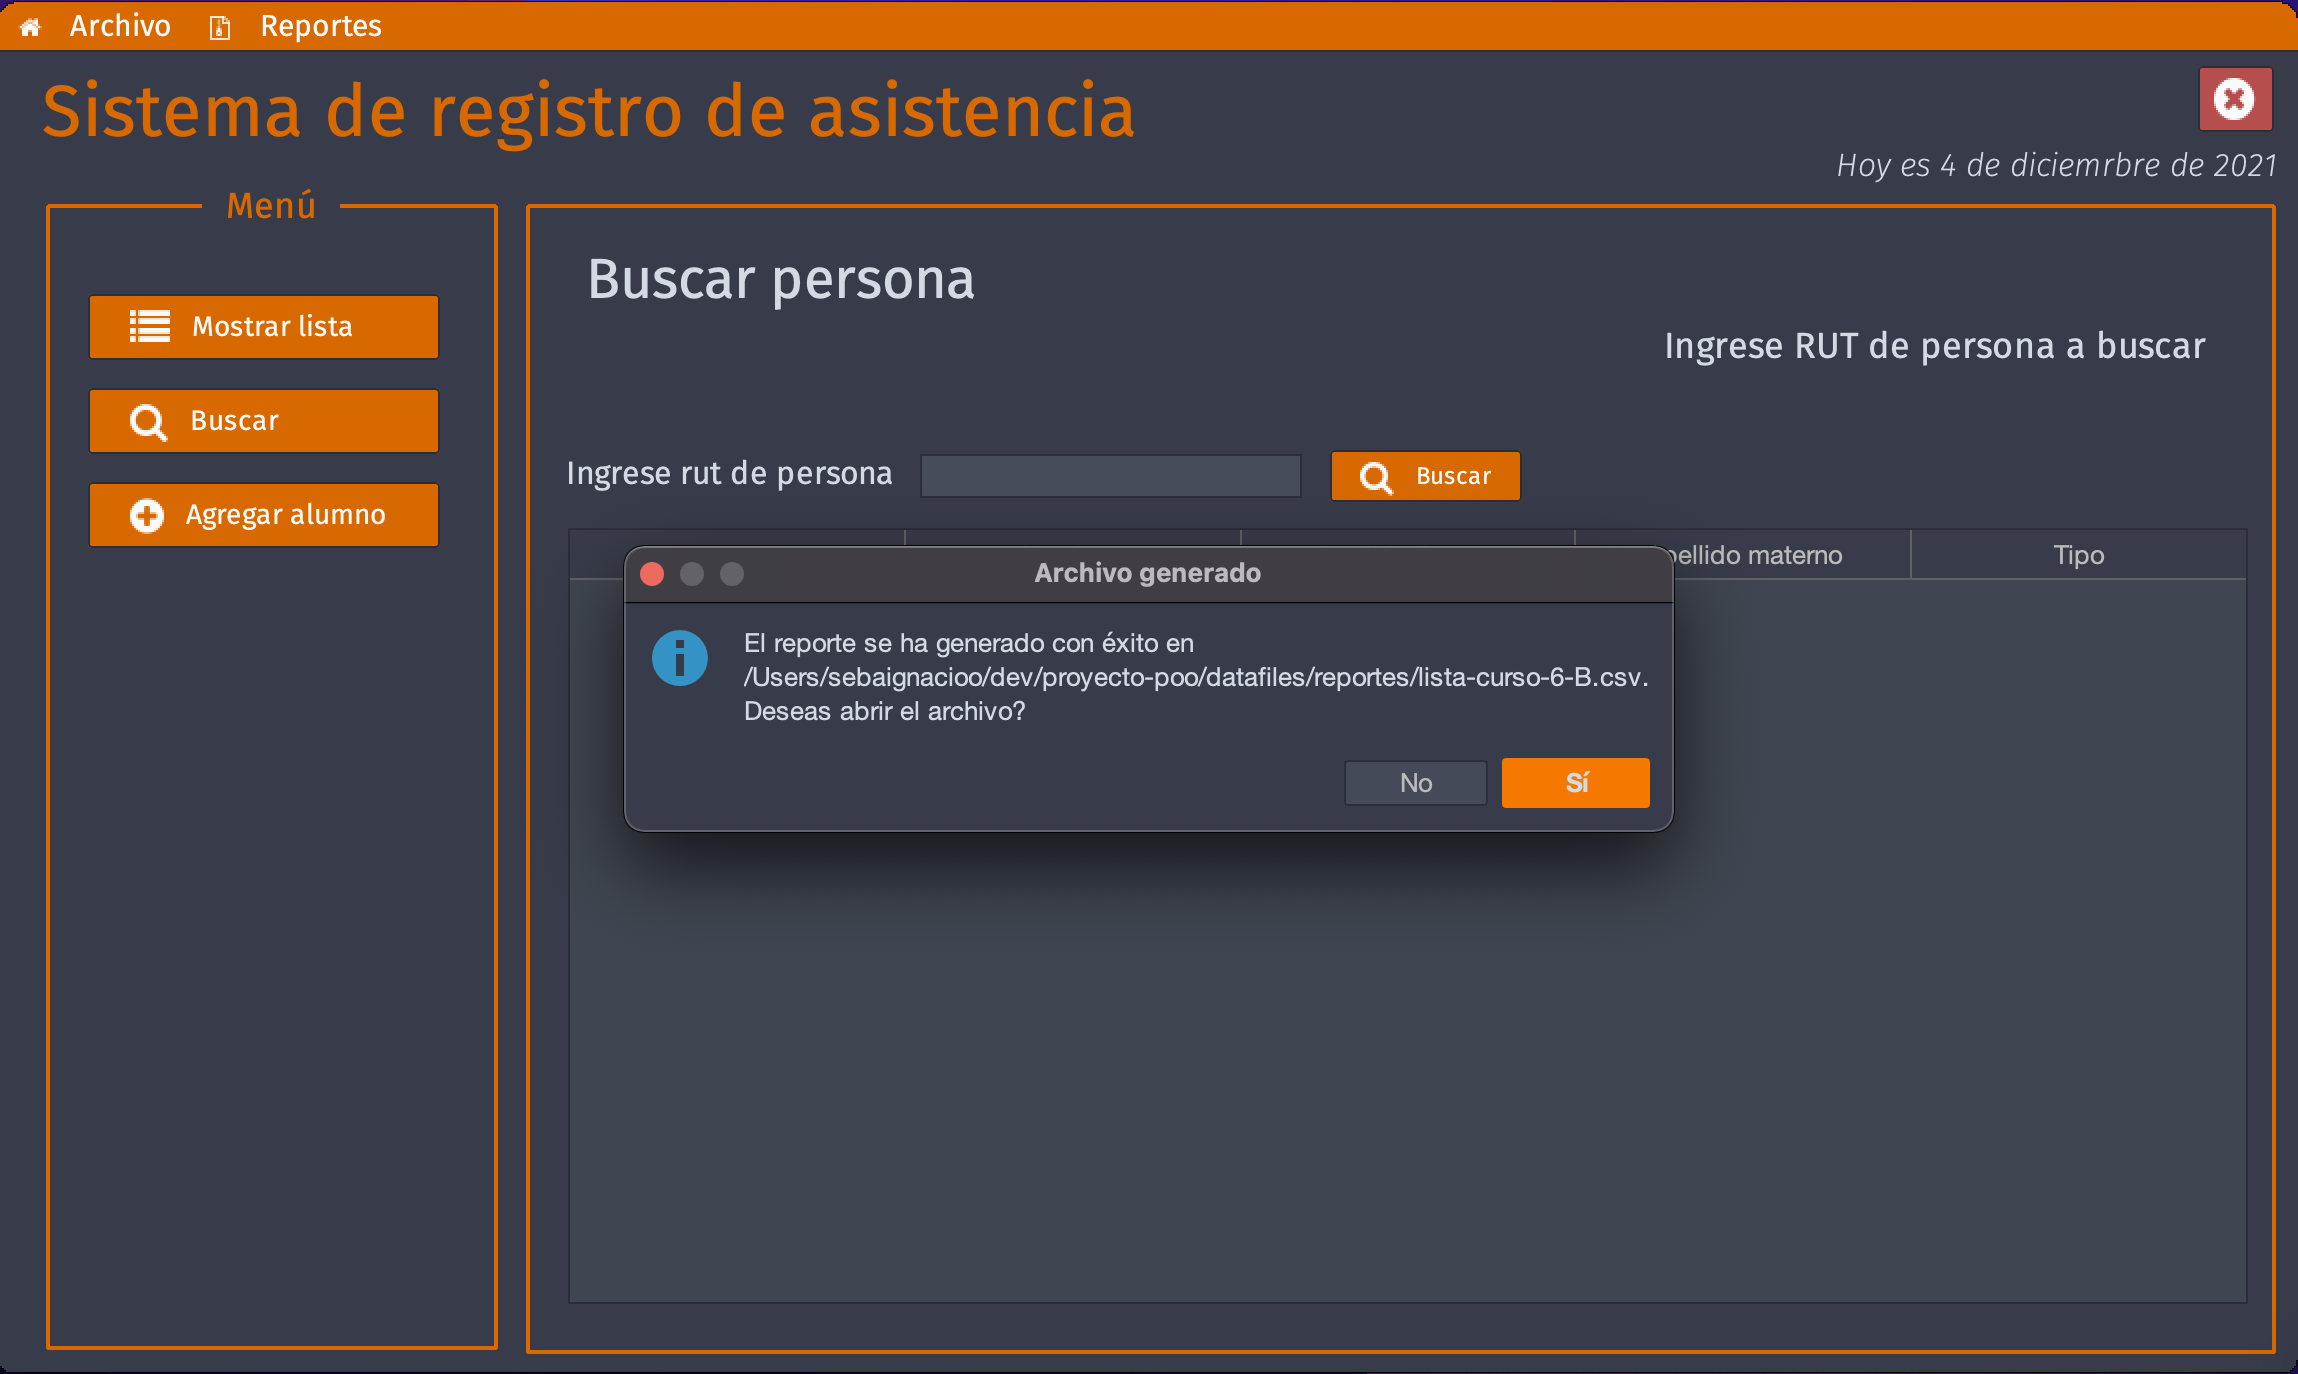
\includegraphics[width=0.95\linewidth]{contents/img/gui/img17}}
    \end{subfigure}
\end{figure}

\clearpage

\subsection{El código fuente debe estar bien modularizado de acuerdo a lo descrito en el informe además de seguir las buenas prácticas de documentación interna y legibilidad}

En el desarrollo de este proyecto, se siguieron las buenas prácticas tanto en los estándares de codificación, como en el desarrollo de la documentación. Más detalles respecto al desarrollo de este proyecto, se puede encontrar más adelante en este mismo informe, al que se puede acceder {\color{MyGreen}\hyperref[subsec:desarrolloapp]{siguiendo este link}}

\subsection{Todas las funcionalidades pueden ser implementadas mediante consola}

Todas las funcionalidades planteadas para el sistema fueron implementadas en la interfaz de consola de comandos (CLI). Solo algunas funcionalidades, indicadas más adelantes en este reporte, fueron implementadas a la interfaz gráfica (GUI).

\subsection{Utilizacion de GitHub (Realización de al menos 3 Commit)}

Respecto a la utilización de la herramienta \textbf{GitHub} para control de versiones, se detalla su uso en el apartado Consideraciones, al que se puede acceder {\color{MyGreen}\hyperref[cons:utilizaciongithub]{siguiendo este link}}.
